
\documentclass{article}

\usepackage{graphicx}
\usepackage{hyperref}
\usepackage{stmaryrd}

\setlength{\parindent}{0in}
\setlength{\textwidth}{160mm}
\setlength{\textheight}{225mm}
\setlength{\topmargin}{8mm}
\setlength{\evensidemargin}{0mm}
\setlength{\oddsidemargin}{0mm}
\sloppy

\newcommand{\hl}{\smallskip\hrule\smallskip}

\pagestyle{empty}
\begin{document}

\setlength{\unitlength}{\textwidth}
\begin{picture}(0,0)(0,-0.05)
\put(0,0){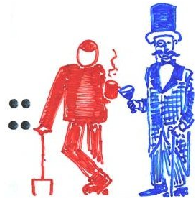
\includegraphics[height=2cm]{semicolon}}
\put(0.5,0.02){\makebox(0,0){\Large \url{http://msp.cis.strath.ac.uk/}}}
\put(0.5,0.06){\makebox(0,0){\Large Mathematically Structured Programming Group}}
\put(0.5,0.10){\makebox(0,0){\Large University of Strathclyde}}
\put(0.5,-0.01){\makebox(0,0){\rule{\textwidth}{0.5pt}}}
\put(1,0){\makebox(0,0)[rb]{
\includegraphics[height=2cm]{strath_science}}}
\end{picture}

\begin{center}
{\Large ``MSP 101'' seminar}
\end{center}

\bigskip

%\bigskip

\begin{center}
  {\Large \bf Simplicial Models for Multi-Agent Epistemic Logic}
\smallskip

J\'er\'emy Ledent\\
MSP group
\end{center}

\begin{quote}
{\em Friday 24 January 2020, 14:00

Room 1310, Livingstone Tower}
\end{quote}

\bigskip

\begin{minipage}{1.0\linewidth}
{
\renewcommand{\thefootnote}{[\arabic{footnote}]} %\footnotemark[1]\footnotetext{[1] ...}
\small \textbf{Abstract:}
\setlength{\parskip}{0.5em}

Epistemic Logic is the modal logic of \emph{knowledge}. It allows one to reason about a finite set of agents who can know facts about the world, and about what the other agents know. The traditional way to interpret epistemic logic formulas is by using \emph{Kripke models}: that is, graphs whose vertices represent the possible worlds, and whose edges indicate the agents that cannot distinguish between two worlds. I will present an alternative kind of model for epistemic logic based on \emph{chromatic simplicial complexes}. Simplicial models are equivalent to Kripke models; thus, this connection uncovers the higher-dimensional geometric nature of knowledge. Finally, I will show how to adapt these geometric models in order to interpret other epistemic notions, such as belief, distributed knowledge, and more.
}
\end{minipage}


\vskip 4cm
\begin{center}

\includegraphics[width=1\textwidth]{glasgow_new}
\end{center}
\end{document}
